% The primes of Z[i] above the primes of Z, in the style of Mumford's drawing (generated by a script).
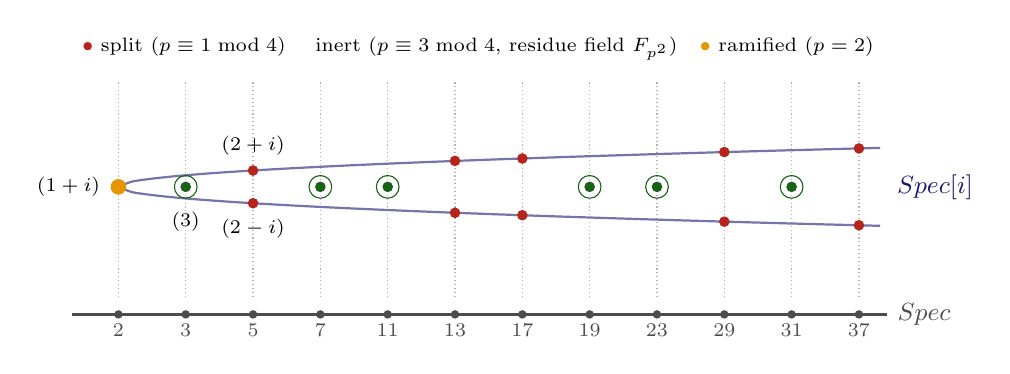
\begin{tikzpicture}[scale=0.9]
\draw[thick,black!70] (0.3,0)--(11.80,0) node[right,font=\small]{$\operatorname{Spec}\Z$};
\fill[black!70] (0.95,0) circle (0.06) node[below,font=\scriptsize]{$2$};
\draw[densely dotted,black!30] (0.95,0.25)--(0.95,3.3);
\fill[black!70] (1.90,0) circle (0.06) node[below,font=\scriptsize]{$3$};
\draw[densely dotted,black!30] (1.90,0.25)--(1.90,3.3);
\fill[black!70] (2.85,0) circle (0.06) node[below,font=\scriptsize]{$5$};
\draw[densely dotted,black!30] (2.85,0.25)--(2.85,3.3);
\fill[black!70] (3.80,0) circle (0.06) node[below,font=\scriptsize]{$7$};
\draw[densely dotted,black!30] (3.80,0.25)--(3.80,3.3);
\fill[black!70] (4.75,0) circle (0.06) node[below,font=\scriptsize]{$11$};
\draw[densely dotted,black!30] (4.75,0.25)--(4.75,3.3);
\fill[black!70] (5.70,0) circle (0.06) node[below,font=\scriptsize]{$13$};
\draw[densely dotted,black!30] (5.70,0.25)--(5.70,3.3);
\fill[black!70] (6.65,0) circle (0.06) node[below,font=\scriptsize]{$17$};
\draw[densely dotted,black!30] (6.65,0.25)--(6.65,3.3);
\fill[black!70] (7.60,0) circle (0.06) node[below,font=\scriptsize]{$19$};
\draw[densely dotted,black!30] (7.60,0.25)--(7.60,3.3);
\fill[black!70] (8.55,0) circle (0.06) node[below,font=\scriptsize]{$23$};
\draw[densely dotted,black!30] (8.55,0.25)--(8.55,3.3);
\fill[black!70] (9.50,0) circle (0.06) node[below,font=\scriptsize]{$29$};
\draw[densely dotted,black!30] (9.50,0.25)--(9.50,3.3);
\fill[black!70] (10.45,0) circle (0.06) node[below,font=\scriptsize]{$31$};
\draw[densely dotted,black!30] (10.45,0.25)--(10.45,3.3);
\fill[black!70] (11.40,0) circle (0.06) node[below,font=\scriptsize]{$37$};
\draw[densely dotted,black!30] (11.40,0.25)--(11.40,3.3);
\draw[thick,MidnightBlue!60] plot[smooth,domain=0.95:11.70,samples=60] (\x,{1.8+0.55*sqrt(\x-0.95)/sqrt(10.75)});
\draw[thick,MidnightBlue!60] plot[smooth,domain=0.95:11.70,samples=60] (\x,{1.8-0.55*sqrt(\x-0.95)/sqrt(10.75)});
\node[right,font=\small,MidnightBlue] at (11.80,1.8) {$\operatorname{Spec}\Z[i]$};
\fill[Orange!90!black] (0.95,1.8) circle (0.11);
\node[font=\scriptsize,anchor=east] at (0.83,1.8) {$(1+i)$};
\fill[ForestGreen!70!black] (1.90,1.8) circle (0.075);
\draw[ForestGreen!70!black] (1.90,1.8) circle (0.16);
\fill[BrickRed] (2.85,2.031) circle (0.075);
\fill[BrickRed] (2.85,1.569) circle (0.075);
\fill[ForestGreen!70!black] (3.80,1.8) circle (0.075);
\draw[ForestGreen!70!black] (3.80,1.8) circle (0.16);
\fill[ForestGreen!70!black] (4.75,1.8) circle (0.075);
\draw[ForestGreen!70!black] (4.75,1.8) circle (0.16);
\fill[BrickRed] (5.70,2.166) circle (0.075);
\fill[BrickRed] (5.70,1.434) circle (0.075);
\fill[BrickRed] (6.65,2.200) circle (0.075);
\fill[BrickRed] (6.65,1.400) circle (0.075);
\fill[ForestGreen!70!black] (7.60,1.8) circle (0.075);
\draw[ForestGreen!70!black] (7.60,1.8) circle (0.16);
\fill[ForestGreen!70!black] (8.55,1.8) circle (0.075);
\draw[ForestGreen!70!black] (8.55,1.8) circle (0.16);
\fill[BrickRed] (9.50,2.291) circle (0.075);
\fill[BrickRed] (9.50,1.309) circle (0.075);
\fill[ForestGreen!70!black] (10.45,1.8) circle (0.075);
\draw[ForestGreen!70!black] (10.45,1.8) circle (0.16);
\fill[BrickRed] (11.40,2.342) circle (0.075);
\fill[BrickRed] (11.40,1.258) circle (0.075);
\node[font=\scriptsize,anchor=south] at (2.85,2.11) {$(2+i)$};
\node[font=\scriptsize,anchor=north] at (2.85,1.49) {$(2-i)$};
\node[font=\scriptsize,anchor=north] at (1.90,1.58) {$(3)$};
\node[font=\scriptsize,align=left,anchor=west] at (0.3,3.75) {\textcolor{BrickRed}{$\bullet$} split ($p\equiv1\bmod 4$)\quad \textcolor{ForestGreen!70!black}{$\circledcirc$} inert ($p\equiv3\bmod4$, residue field $\mathbb F_{p^2}$)\quad \textcolor{Orange!90!black}{$\bullet$} ramified ($p=2$)};
\end{tikzpicture}
